\documentclass[10pt,landscape,twocolumn]{article}

\usepackage{lscape}
\usepackage[english]{babel}
\usepackage[utf8]{inputenc}
\usepackage{fullwidth}

\usepackage{tikz}
\usetikzlibrary{calc}
\usepackage{fancyhdr}
\pagestyle{fancy}

\renewcommand{\footrulewidth}{1pt}
\fancyfoot[C]{\thepage}

\renewcommand{\headrulewidth}{1pt}
\fancyhead[L]{ACM ICPC}

\begin{document}

\begin{center}
	\Large ICPC Training Material : Data Structures, Algorithms and Theorems 
\end{center}

\tableofcontents

\section{Data Structures}

\subsection{Elementary Data Structures}
In Computer Science, in order to treat and store data, it first needs to be structured. Hence, multiple data structures were created : Array, Hash, Queue, Tree and multiple others.

\subsubsection{Array}
The array is the most used data structure. It consists on a collection of values, such as each value is identified by at least one index. 
\begin{center}
	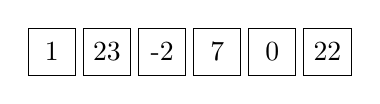
\begin{tikzpicture}
	\coordinate (s) at (0,0);
	\foreach \num in {1,23,-2,7,0,22}{
		\node[minimum size=6mm, draw, rectangle] at (s) {\num};
		\coordinate (s) at ($(s) + (0.7,0)$);
	}
	\end{tikzpicture}
\end{center}
Arrays are useful because they exploit the addressing logic of computers. Generally, the memory is a one-dimensionnal array of words, whose indices are the addresses.

\subsubsection{Stack}

The stack is a data structure 
\subsubsection{Queue}
\subsubsection{Heap}
\subsubsection{Hash}
\subsubsection{Trees}

\subsection{Advanced Data Structures}

\subsubsection{Priority queues}
\subsubsection{Fenwick Tree}
\subsubsection{K-D Tree}
\subsubsection{Interval Tree}

\section{Algorithms}

\subsection{Sorting and Searching}

\subsubsection{Binary Search}
\subsubsection{Merge Sort}
\subsubsection{Quick Sort}
\subsubsection{Heap Sort}

\subsection{String manipulation}
\subsubsection{KMP Algorithm}
\subsubsection{Rabin Karp}
\subsubsection{Z Algorithm}
\subsubsection{Aho Corasick Algorithm}

\subsection{Graph Algorithms}
\subsubsection{Breadth First Search}
\subsubsection{Depth First Search}
\subsubsection{Djikstra's Algorithm}
\subsubsection{Floyd Warshall's Algorithm}
\subsubsection{Prim's Algorithm}
\subsubsection{Kruskal's Algorithm}
\subsubsection{Topological Sort}
\subsubsection{Johnson's algorithm}


\subsection{Network Flow Algorithms}
\subsubsection{Ford Fulkerson Algorithm}
\subsubsection{Dinic's Algorithm}
\subsubsection{Hopcroft Karf Algorithm}
\subsubsection{Gomory-Hu Algorithm}
\subsubsection{Stoer-Wagner Algorithm}

\subsection{Geometrical Algorithms}
\subsubsection{Convex hull Algorithm}
\subsubsection{Graham scan Algorithm}
\subsubsection{Bentley-Ottmann Algorithm}
\subsubsection{Rotating calipers}

\section{Mathematics}

\subsection{Number Theory}
\subsubsection{Lucas Theorem}
\subsubsection{Chinese remainder Theorem}
\subsubsection{Primality test}
\subsubsection{Sieve of Eratosthenes}

%\subsection{Combinatorics}

\end{document}
